% !TEX root =  master.tex
\chapter{Projektplanung}
	
	\section[Projektdefinition]{Projektdefinition {\hfill \normalsize Milena Zahn}}
	Das Ziel des Projektes \enquote{\ac{ICS}} ist die Entwicklung eines Prototypen für die Online-Reservierung von Kino-Tickets. Das Projekt wird mit der vorliegenden Seminararbeit dokumentiert. Ergebnis soll ein lauffähiger Prototyp sein, mit dem es möglich ist Sitze für eine Filmvorstellung erfolgreich zu reservieren. Mit dem Vorlesungsbeginn am 26.11.2018 wird das Projekt gestartet und endet mit der Abschlusspräsentation am 12.02.2019.
	
	\section[Projektbeteiligte]{Projektbeteiligte{\hfill \normalsize Milena Zahn}}
	An diesem Projekt \ac{ICS} arbeiten acht Personen des Kurses WWI 17 SE B der Dualen Hochschule Baden-Württemberg in Mannheim. Im Rahmen der Lehrveranstaltung \enquote{Fallstudie} des Moduls \enquote{Umsetzung der Methoden der Wirtschaftsinformatik} legen folgende Studenten ihre Prüfungsleistung ab:
	\begin{singlespacing}
	\begin{itemize}
		\item Dutzi Jonas, Matrikelnummer: 6681598
		\item Keller Sandra, Matrikelnummer: 6046520 
		\item Köhler Dennis, Matrikelnummer: 8900967 
		\item Sandig Martin, Matrikelnummer: 8857640 
		\item Waage Felix, Matrikelnummer: 3459154 
		\item Werner Yvonne, Matrikelnummer: 8519757 
		\item Westphal Fabio, Matrikelnummer: 6198411  
		\item Zahn Milena, Matrikelnummer: 7488221 
	\end{itemize}
	\end{singlespacing}

	\section[Feasibility Study]{Feasibility Study{\hfill \normalsize Milena Zahn}}
	Bevor das Projekt \ac{ICS} gestartet ist, wurde zuerst eine Feasibility Study, dt. Machbarkeitsstudie, durchgeführt. Es wurde geprüft, ob alle erforderlichen Voraussetzungen für das Projekt vorhanden sind. Die in dem ersten Studienjahr vermittelten programmiertechnischen sowie methodischen Grundlagen werden angewandt. Durch die Lehrveranstaltung \enquote{Systemanalyse und -entwurf} des zweiten Semesters wurden alle notwendigen Kompetenzen zur objektorientierten Analyse und Entwurf erworben. Durch das Modul \enquote{Programmierung und Programmiertechniken} des ersten und zweiten Semesters kann man Erfahrungen in der Programmiersprache Java voraussetzen. Vor dem Projektstart wurden die Rahmenbedingungen, unter denen das Projekt laufen soll, von dem Dozenten gegeben. Des Weiteren wurde innerhalb der Gruppe besprochen, inwiefern das Projekt in der gegeben Zeit umgesetzt werden kann. Der Prozess, dass unterschiedliche Personen sinnvoll zusammenwirken und vielfältige Fähigkeiten genutzt sowie ausgeglichen werden, stellt eine Herausforderung dar. Die Verständigung und Absprachen der in einem cross-funktionalen Team zusammenarbeiten Personen muss reibungslos funktionieren, damit der Informationsaustausch und die Verteilung der Aufgaben sich positiv auf das Projektergebnis auswirken.
	
	Unter Berücksichtigung der Bedingungen dieses Projekts ist vor allem der enge Zeitrahmen auffällig. Das Projektmanagement ist somit neben der Implementierung des Kino-Reservierungstools an sich eine sehr wichtige Aufgabe. Parallel zu diesem Projekt müssen weitere Prüfungsleistungen sowie Vorlesungen von anderen Modulen des dritten Semesters absolviert und demnach mit berücksichtigt werden. Um diese einzuplanen und ein erfolgreiches Projekt abzuschließen, ist eine Projektplanung essentiell. Laut Christoph Wegmann steht \enquote{Planung und Projekterfolg [...] in direktem Zusammenhang}\autocite[][S. 73]{projektmanagement}. Aus diesen Gründen wurde das Projektmanagement von Anfang an von allen Teammitgliedern durchgeführt und beachtet.
	
	\section[Zeitplanung]{Zeitplanung{\hfill \normalsize Milena Zahn}} \label{projektplan}
	\subsection{Projektzeitplan}
	\enquote{Um die Ergebnisse [...] termingerecht zu erreichen, ist eine entsprechend gute Zeitplanung unabdingbar}\autocite[][S. 90]{projektmanagement}.
	In Abbildung \vref{fig:projektablauf} wird der Projektablauf, der zu Beginn des Projektes aufgestellt wurde, dargestellt. Das Projekt beginnt am 26.11.2018 und endet am 12.02.2019. Innerhalb dieser zwölf Wochen sind drei Iterationen vorgesehen. Im Rahmen einer kurzen Präsentation in KW51 2018 und KW4 2019 werden die in der jeweiligen Iteration erarbeiteten Ergebnisse dem Dozenten sowie dem Kurs vorgestellt. Ziel dieser Präsentationen ist es, den aktuellen Projektstatus vorzustellen und Feedback einzuholen. Außerdem dienen diese Präsenzen dazu, Fragen zu stellen und sonstige Hindernisse zu klären. 
	\begin{figure}[H]
		\centering 
		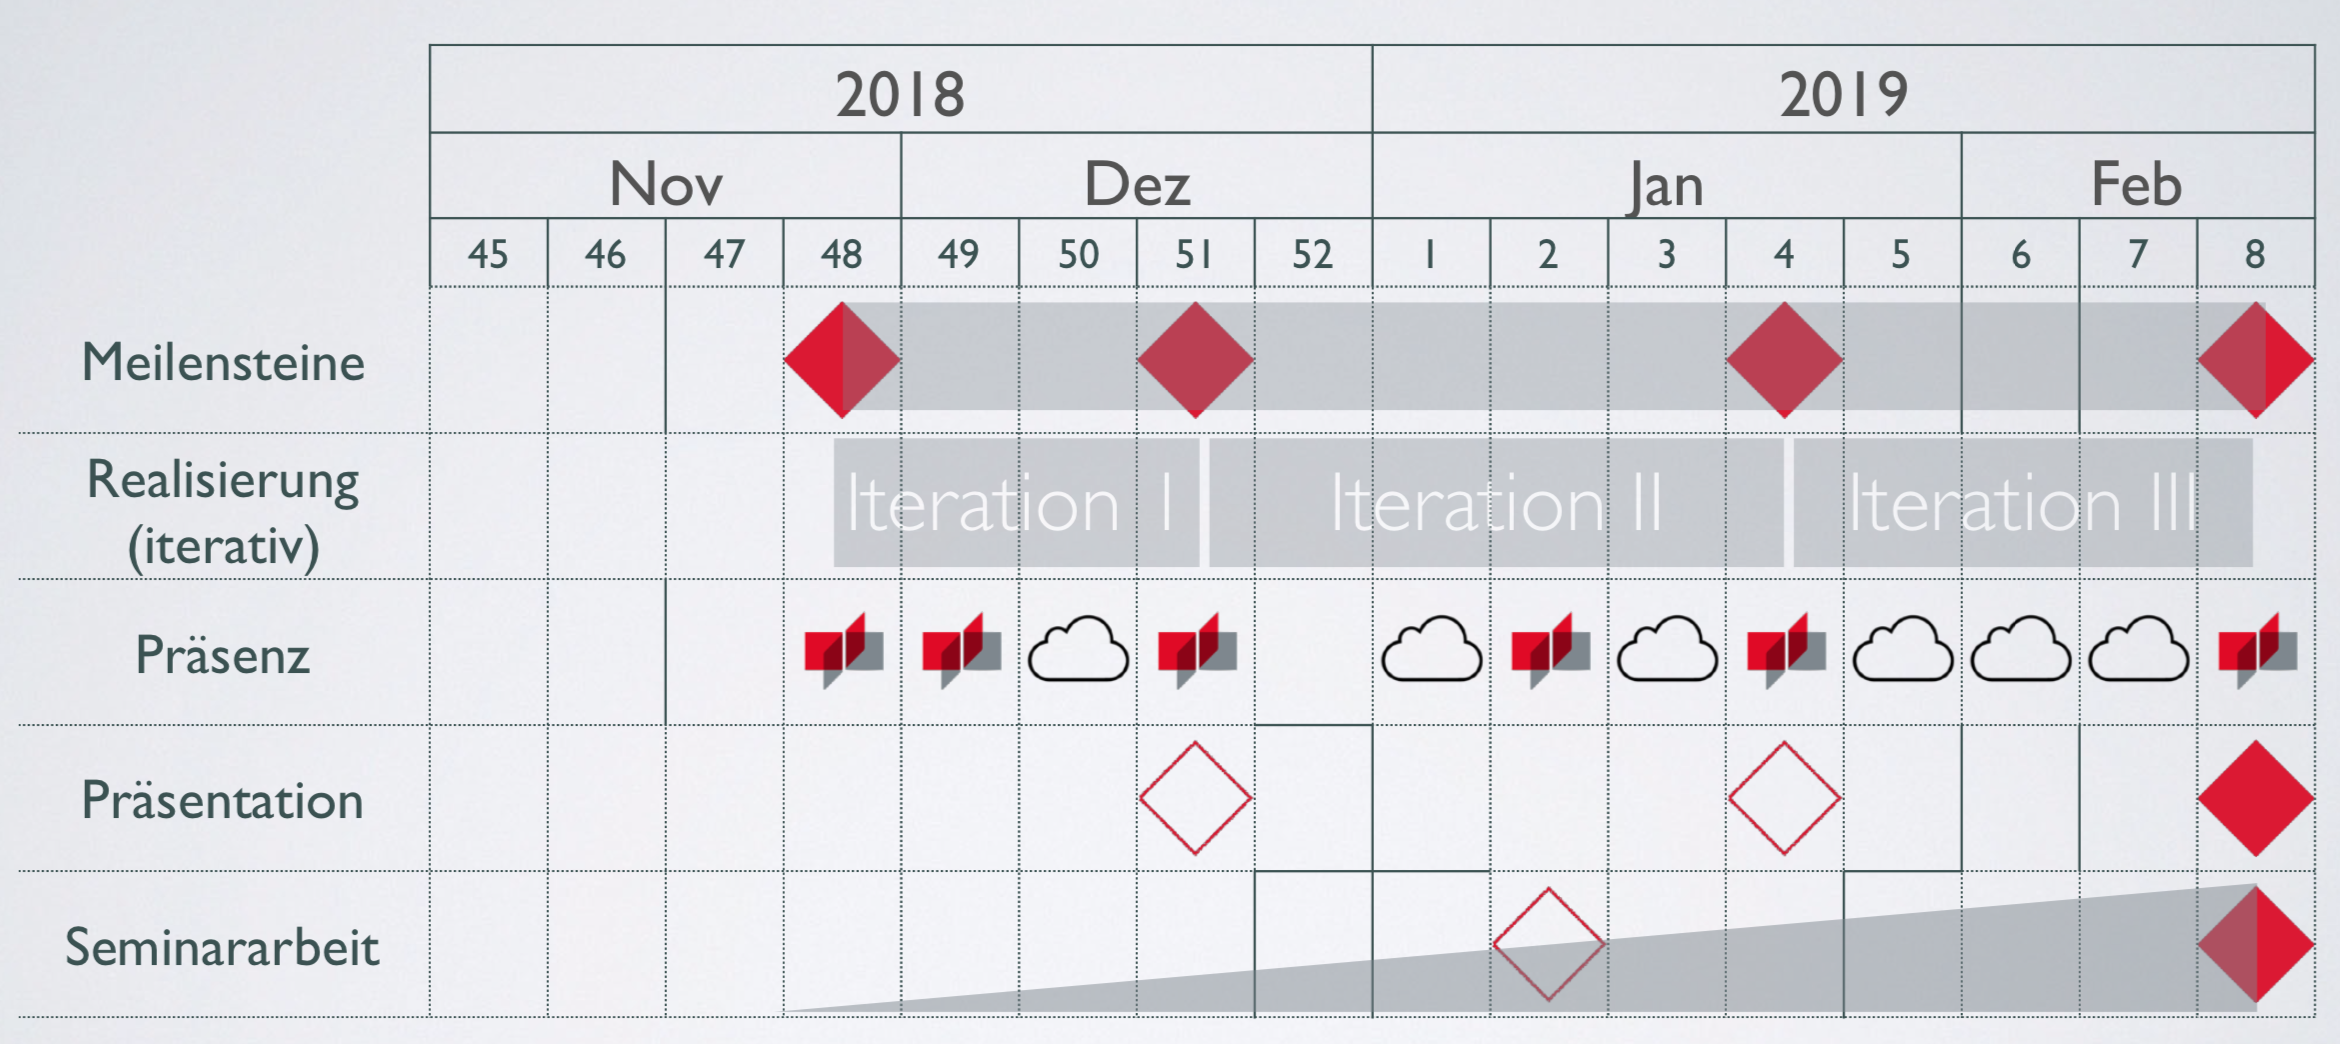
\includegraphics[width=12cm]{img/geplanterProjektablauf.png}
		\captionsetup{format=hang}
		\caption[Geplanter Projektablauf ]{\label{fig:projektablauf} Geplanter Projektablauf \\ Quelle: Skript, Gregor Tielsch }
	\end{figure}
	
	\subsection{Projektplanung mit Gantt Diagramm}
	Der Projektplan ist das zentrale Dokument des Projektmanagements, da er den Projektfortschritt unterstützt und alle Aufgaben enthält, die innerhalb dieses Projektes zu erledigen sind. Diese Dokumentation garantiert ein erfolgreiches und optimales Projektmangement. Das Gantt Diagramm ist eine Tabelle bestehend aus geplanten Vorgängen sowie Meilensteinen, die in einem dahinter dargestellten Kalender über Balken eingezeichnet werden\autocite[Vgl.][S. 107]{projektmanagement}. Heutzutage ist dieses Instrument des Projektmanagements die gängigste Methode, um Aktivitäten zeitbezogen zu dokumentieren. Um die Vorteile dieser Methode zu nutzen, wurde entschieden ein daran angelehntes Modell einzuführen. Damit der Projektplan jedem Teammitglied jederzeit zur Verfügung steht und um von der Nützlichkeit eines Online-Tools zu profitieren, wurde entschieden das Gantt Diagramm mit der Planungssoftware \enquote{Tom's Planner}\footnote{https://www.tomsplanner.de} zu erstellen.
	Das Projektmanagement wurde für die gesamte Projektzeit durchgeführt. Die Aktivitäten des Projekts sind in der Abbildung \vref{fig:projektplan} gruppiert dargestellt. Das Gantt Diagramm wurde stets während der Durchführung des Projektes gepflegt, um den aktuellen Projektfortschritt in einer übersichtlichen Darstellung zu visualisieren. In regelmäßigen Projektsitzungen wurde der Projektfortschritt über das Gantt Diagramm sowie die Meilensteile überwacht und dokumentiert. So ist der Projektstatus jederzeit transparent und für alle Teammitgliedern ersichtlich. Dadurch kann gegebenenfalls eingegriffen werden, wenn Meilensteine nicht erreicht werden und das Projekt in Gefahr läuft in Verzug zu geraten.  
	 Zu Beginn des Projektes wurden die Meilensteine in Orientierung an den Projektablaufplan Abbildung \vref{fig:projektablauf} angelegt. 
	\begin{figure}[H]
		\centering 
		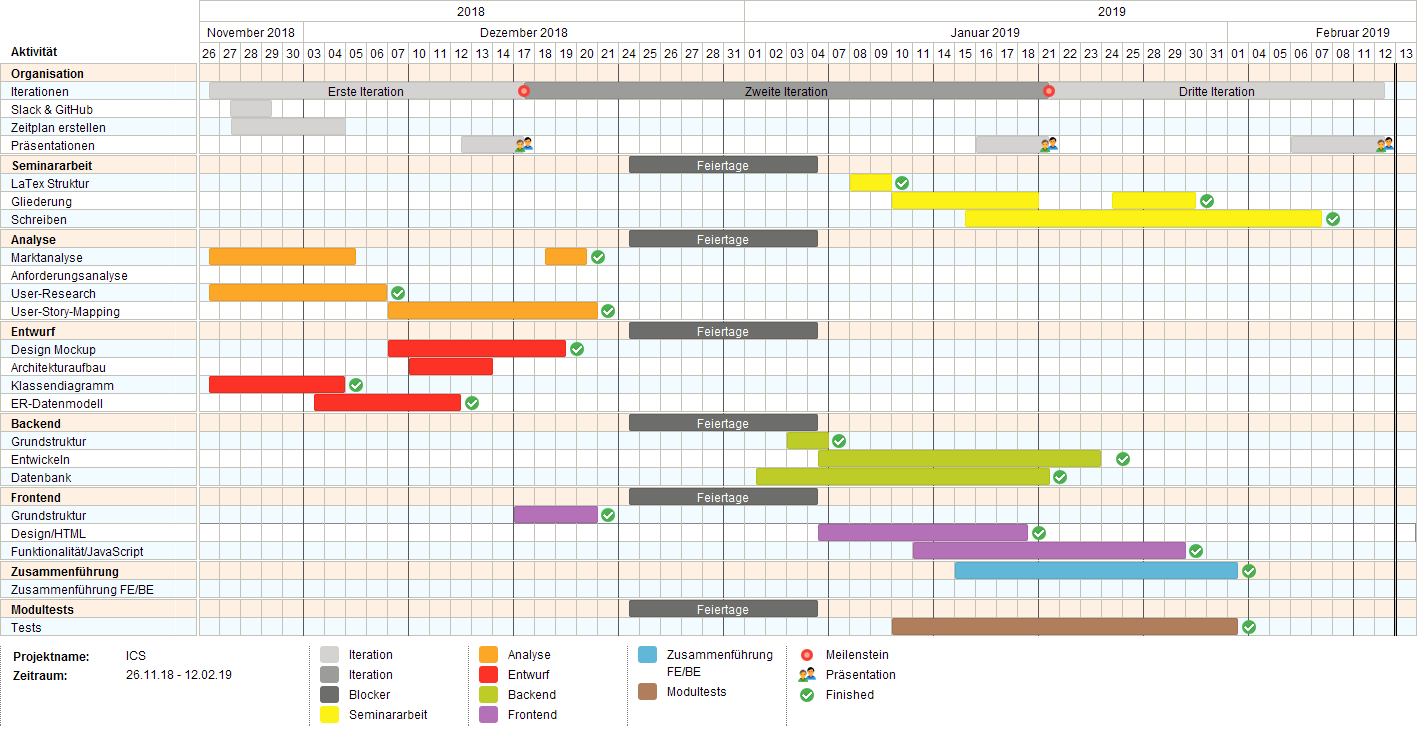
\includegraphics[width=14cm]{img/projektplan.png}
		\captionsetup{format=hang}
		\caption[Projektplan]{\label{fig:projektplan} Projektplan ICS, Gantt-Diagramm \\ Quelle: Tom's Planner}
	\end{figure}
	Die aktuell bearbeiteten Aufgaben wurden kontinuierlich in das Gantt Diagramm eingetragen, damit eine Übersicht entsteht, wann und wie lange an der jeweiligen Aufgabe gearbeitet wurde. Zunächst wurden einige organisatorische Aufgaben erledigt sowie ein Organisations-Tool eingerichtet. Die Organisation des Teams wird in Kapitel \vref{teamorga} genauer erläutert. Die Analyse (Kapitel \vref{analyse}) sowie der Entwurf (Kapitel \vref{entwurf}) wurden in der ersten Interation erarbeitet. Wobei die Marktanalyse in der zweiten Iteration erneut durchgeführt wurde, da zu diesem späteren Zeitpunkt neue Probleme aufgetreten sind. Nachdem das Grundkonzept der Anwendung durch ein Mockup und dem Design der Softwarearchitektur festgelegt wurde, konnte das Backend und das Frontend entwickelt. Dies wird im Kapitel \vref{umsetzung} detaillierter erklärt. In der zweiten und letzen Iteration wurde parallel zu der Entwicklung die Seminararbeit geschrieben. Gegen Ende der dritten Iteration wurde schließlich der Fokus auf die Präsentation sowie die Fertigstellung der Seminararbeit gelegt. Das Projekt endet am 12.02.2019 mit dem letzten Meilenstein \enquote{Abschlusspräsentation}.
	
	
	\section[Teamorganisation]{Teamorganisation{\hfill \normalsize Milena Zahn}} \label{teamorga}
	Eine wichtige Kompetenz innerhalb dieses Projektes ist es, sich selbst sowie das Team zu organisieren, um in dem begrenzten Zeitraum mit den gegebenen Resssourcen das Projektziel zu realisieren. Die Effizienz des Informationsaustausches und der Kommunikation innerhalb des Teams bestimmt wesentlich dessen Erfolg mit. Eine Hauptaufgabe in Projekten ist somit die Kommunikation\autocite[Vgl.][S. 207]{projektmanagement}. Insbesondere bei den zeitlich begrenzten Aufgaben und temporären Organisationsstrukturen ist ein reibungsloser Austausch, der jedes Projektmitglied mit den essentiellen Informationen versorgt, entscheidend. Aus diesem Grund wurde das Kommunikationstool \enquote{Slack}\footnote{https://slack.com/} gewählt. Die Projektbeteiligten sind alle mit dem Programm, unter anderem durch die Lernveranstaltung \textit{Systemanalyse und -entwurf} und durch die Praxisphasen in dem Unternehmen, vertraut. Dadurch kann eine Einarbeitungszeit eingespart werden kann. Für das Projekt wurde ein eigener Workspace, auf den alle Projektbeteiligten zugreifen können, angelegt. Kurze Teamabsprachen sowie Fragestellungen innerhalb des Teams, konnten damit schnell und unkompliziert geklärt werden. Ein weiterer Vorteil von Slack ist die Transparenz, die durch die verschiedenen, offenen Channels gegeben wird. Ein weiterer Vorteil ist die Dauerhaftigkeit der besprochenen Themen und beschlossenen Entscheidungen. Dadurch werden Entscheidungen dokumentiert und können bei Unklarheiten jederzeit wieder eingesehen werden. Durch \enquote{Slack} wurde damit ein stetiger, unkomplizierter Dialog unter den Teammitgliedern ermöglicht, der die Bearbeitung des Projektes unterstützt und vereinfacht hat.
	
	\section[Projektabschluss]{Projektabschluss{\hfill \normalsize Milena Zahn}} 
	Der Projektabschluss ist die letzte Phase für das Projekt. Es wird deutlich, ob die Ziele erreicht wurden und ein Projektreview erstellt. Dies wird in dem Kapitel \vref{Ausblick}, mit Fokus auf das Projektreview und Lessons Learned, und in dem Kapitel \vref{Evaluation}, mit Fokus auf die Zielerreichung und der Potenziale, ausgeführt. Das Projekt wird durch eine Abschlusspräsentation, in der der fertige Protoyp vorgestellt wird, sowie der vorliegenden Seminararbeit abgeschlossen. Die Projektabschlussbewertung wird schließlich von Herrn Gregor Tielsch, Dozent der Lehrveranstaltung \enquote{Fallstudie}, durchgeführt.